\documentclass[tikz, border=8pt]{standalone}
\usepackage{amsmath}

\begin{document}
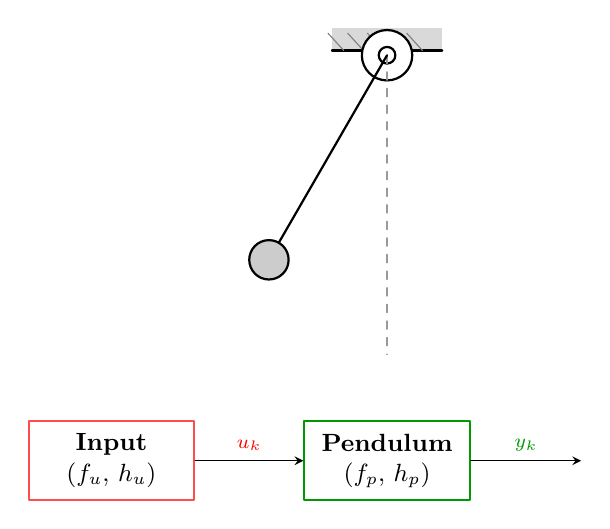
\begin{tikzpicture}[
  line cap=round, line join=round, >=stealth,
  blk/.style={draw, thick, minimum width=2.1cm, minimum height=1.0cm,
              align=center, fill=white, font=\small}
]

  % ── Physical pendulum ─────────────────────────────────────────────────────

  % Wall mount
  \fill[black!15] (-0.7, 0.06) rectangle (0.7, 0.35);
  \draw[thick] (-0.7, 0.06) -- (0.7, 0.06);
  \foreach \xi in {-0.55,-0.30,-0.05,0.20,0.45}
    \draw[thin, black!50] (\xi, 0.06) -- ++(-0.20, 0.22);

  % Motor (outer circle + inner pin)
  \filldraw[fill=white, draw=black, thick] (0,0) circle (0.32);
  \filldraw[fill=white, draw=black, thick] (0,0) circle (3pt);

  % Dashed vertical
  \draw[dashed, black!40, thin] (0,0) -- (0,-3.8);

  % Rod
  \draw[thick] (0,0) -- (-1.5, -2.598);

  % Bob
  \filldraw[fill=black!20, draw=black, thick] (-1.5, -2.598) circle (0.25);

  % ── Blocks ────────────────────────────────────────────────────────────────

  \node[blk, draw=red!70]         (inp)   at (-3.5, -5.15)
      {\bfseries Input\\\normalfont$(f_u,\,h_u)$};
  \node[blk, draw=green!60!black] (plant) at (0,    -5.15)
      {\bfseries Pendulum\\\normalfont$(f_p,\,h_p)$};

  % u_k: Input → Pendulum
  \draw[->] (inp.east) -- (plant.west)
    node[midway, above, font=\scriptsize\itshape, red] {$u_k$};

  % y_k: Pendulum → output
  \draw[->] (plant.east) -- ++(1.4, 0)
    node[midway, above, font=\scriptsize\itshape, green!60!black] {$y_k$};

\end{tikzpicture}
\end{document}
